\documentclass[12pt,fleqn]{article}\usepackage{../../common}
\begin{document}
Sezonsallık, Trend Çıkartmak, Değişim Noktası



\begin{minted}[fontsize=\footnotesize]{python}
def model_compute(X, coef):
   degree = len(coef)-1
   curve = [np.sum([coef[-1]] + [x**(degree-d)*c for d,c \
            in enumerate(coef[:-1])]) for x in X]
   return curve
\end{minted}


\begin{minted}[fontsize=\footnotesize]{python}
from pandas import datetime
def parser(x):
    return datetime.strptime( '190'+x, '%Y-%m' )
    
df = pd.read_csv('shampoo-sales.csv', header=0, index_col=0, \
     parse_dates=True, date_parser=parser)

X = np.array(range(len(df))).reshape(-1)
y = df.values.reshape(-1)
degree = 1
coef = np.polyfit(X, y, degree)
df['Model']  = model_compute(X, coef)
df.plot()
plt.savefig('tser_022_de_01.png')
\end{minted}

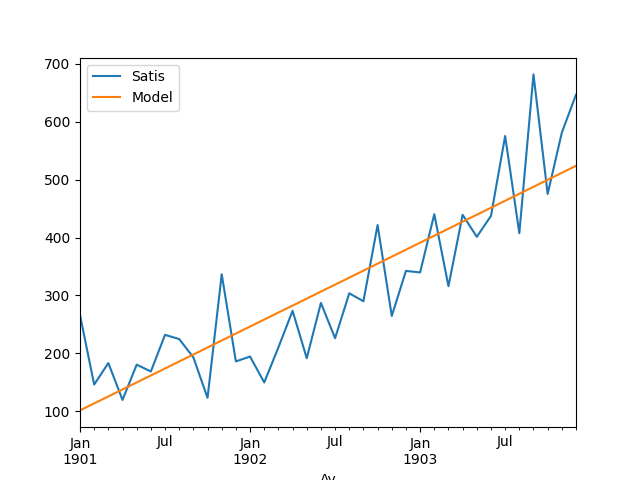
\includegraphics[height=6cm]{tser_022_de_01.png}


\begin{minted}[fontsize=\footnotesize]{python}
detrended = df.Sales-df.Model
detrended.plot()
plt.savefig('tser_022_de_03.png')
\end{minted}

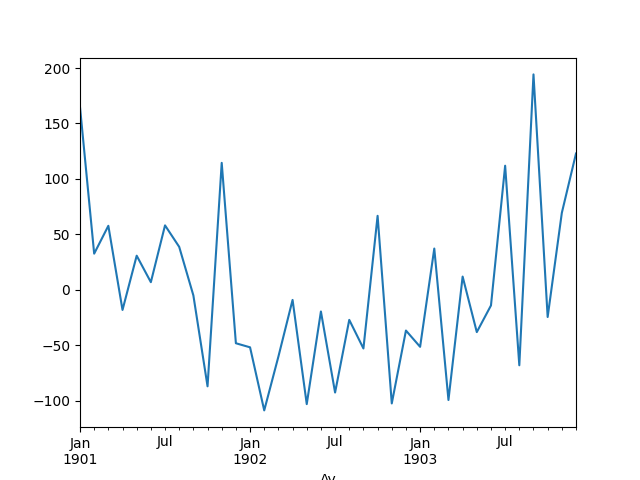
\includegraphics[height=6cm]{tser_022_de_03.png}



\begin{minted}[fontsize=\footnotesize]{python}
import pandas as pd
df = pd.read_csv('daily-min-temperatures.csv', header=0,\
                 index_col=0, parse_dates=True)
X = [i%365 for i in range(0, len(df))]
y = df.values
degree = 4
coef = np.polyfit(X, y, degree)
df['Model']  = model_compute(X, coef)
df.plot()
plt.savefig('tser_022_de_02.png')
\end{minted}


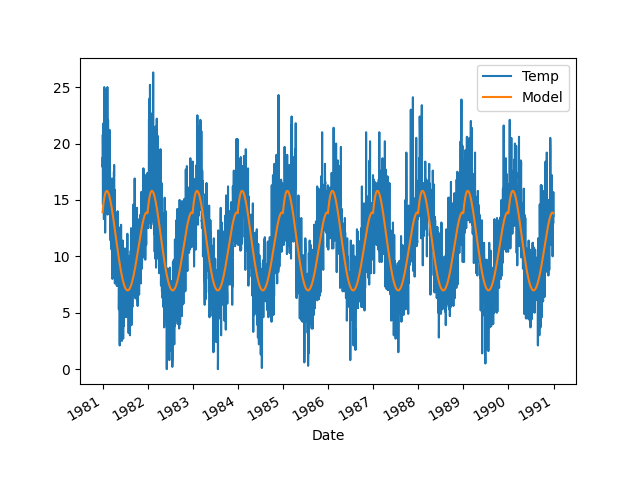
\includegraphics[height=6cm]{tser_022_de_02.png}

\begin{minted}[fontsize=\footnotesize]{python}
detrended = df.Temp-df.Model
detrended.plot()
plt.savefig('tser_022_de_04.png')
\end{minted}


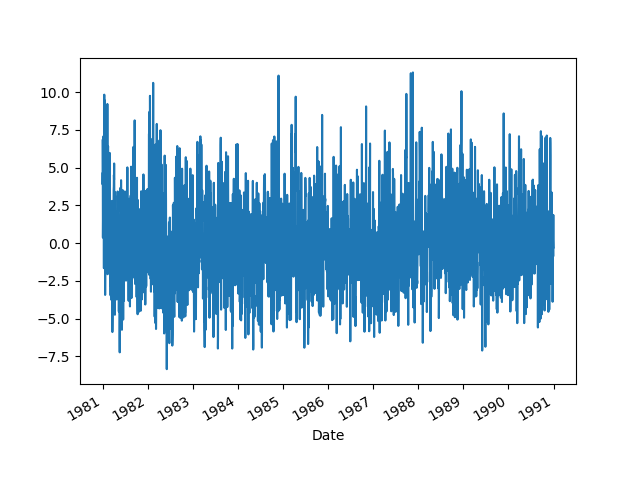
\includegraphics[height=6cm]{tser_022_de_04.png}





 












Kaynaklar

[1] Brownlee, {\em Introduction to Time Series Modeling with Python}

\end{document}
